\newcommand{\ww}{0.64}
%
\section{Experiments and Results}
\label{sec:First}
%
 In this section we present results from our algorithm both in simulation and with a real robotic system. We test different aspects of our algorithm: a) learning the associated meaning of feedback instruction words while learning a new task, b) extending it for the case of guidance words, c) combining learning from unknown instructions with pre-defined signals of known meanings, and d) reusing learnt instruction-to-meaning mapping for the learning of a new task.
%
\subsection{Experimental System}
\label{sec:ExperimentalSetup}
%
We construct a small size pick-and-place task with a real robot. This robot is going to be programmed using a natural speech interface whose words have an unknown meaning and are \textbf{not} transformed into symbols via a voice recognizer. The robot has a prior knowledge about the distribution of possible tasks.% and knows how to accept human instructions.
The interaction between the robot and the human is a turn taking social behavior: the robot performs an action and waits for a feedback, or guidance, instruction to continue. This allows to synchronize a speech wave with its corresponding pair of state and action. The experimental protocol is summarized in figure~\ref{bloc}.
%
\begin{figure}[!htbp]
	\centering
		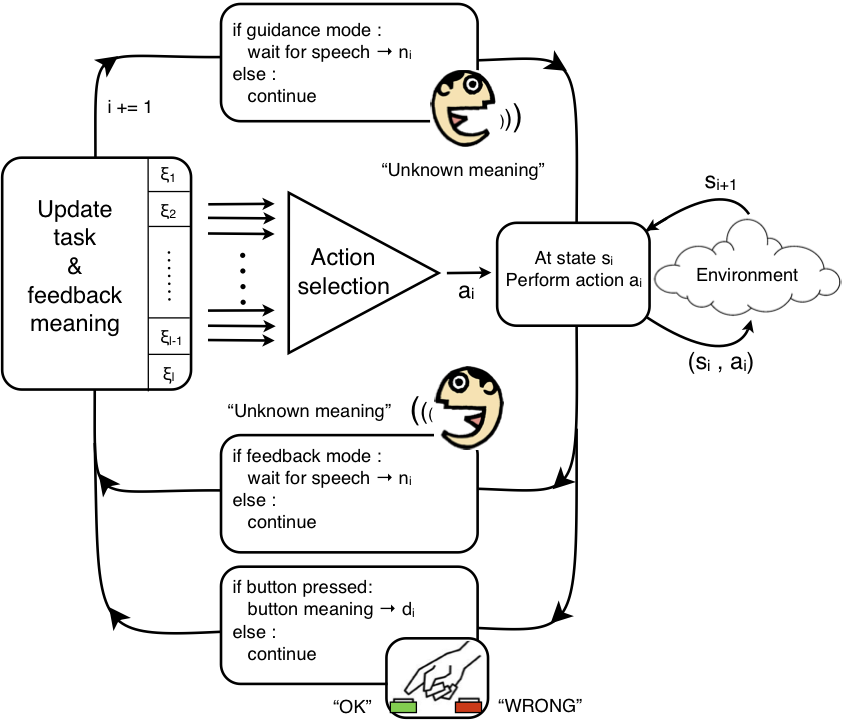
\includegraphics[width=\columnwidth]{images/bloc4.png}
	\caption{Experimental protocol showing the interaction between the teacher and the learning agent. The agent has to learn a task and the meaning of the instructions signals provided by the user, here recorded speech. The teacher can use guidance or feedback instructions but also has access to buttons of known meaning for the robot.}
	\label{bloc}	
\end{figure}
%
\subsubsection{Robotic System}
\label{sec:RoboticSystem}
%
We consider a six d.o.f. robotic arm and gripper that is able to grasp, transport and release cubes in four positions. We used a total of three cubes that can form towers of two cubes.  The robot has 4 actions available: \textit{rotate left}, \textit{rotate right}, \textit{grasp cube} and \textit{release cube}. The state space is discrete and defined as the location of each object, including being on top of another or in the robot's hand. So for a set of 3 objects we have 624 different states. Figure~\ref{setup} shows the robot grasping the orange cube. 
%
\begin{figure}[!htbp]
	\centering
		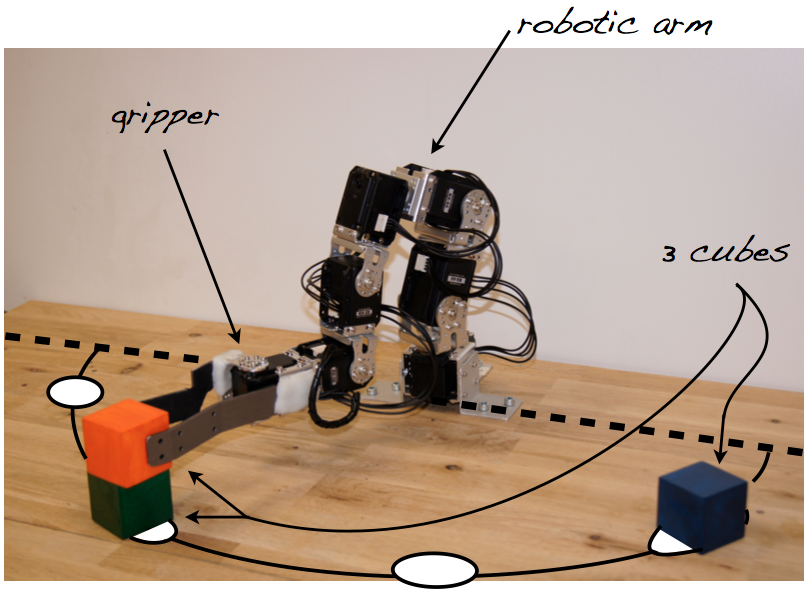
\includegraphics[width=0.8\columnwidth]{images/setup4.png}
	\caption{Robotic System. A six d.o.f robotic arm and gripper learning to perform a pick-and-place task with three cubes.
	        %An example of cubes' configuration which can be described as: \emph{"orange cube is on top of green cube in position 3, blue cube is in position 1 and the robot is grasping the orange cube"}.
	        }
	\label{setup}
\end{figure}
%
\subsubsection{Task Representation}
\label{sec:TaskRepresentation}
%
We assume that for a particular task $\xi$ we are able to compute a policy $\pi$ representing the optimal actions to perform in every state. One possibility is to use \textit{Markov Decision Processes} (MDP) to represent the problem \cite{sutton1998reinforcement}. From a given task $\xi$ represented as a reward function we can compute the corresponding policy using, for instance, \textit{Value Iteration} \cite{sutton1998reinforcement}. In any case, our algorithm does not make any assumption about how tasks are represented.

For this particular representation we assume that the reward function is sparse and so we can generate possible tasks by sampling sparse reward functions. Similarly to \textit{Bayesian Inverse Reinforcement Learning} \cite{Ramachandran07ijcai} the robot learns the task by choosing among the possible space of rewards the most likely one. We approximate this process using a finite set of task hypothesis representing all the reward functions consisting of a unitary reward in one state and no reward in all the others. In other words the task is to reach one, yet unknown, of the 624 states of the MDP.

Under this formalism the action selection at runtime can be done in different ways. As different sampling methods can lead to different learning behaviors, we will compare two different methods: random and  $\epsilon$-greedy. When following random action selection the robot does not use its current knowledge of the task and randomly selects actions. Whereas with $\epsilon$-greedy method the robot performs actions according to the current belief of what the task is, i.e. following the policy corresponding to the most likely task hypothesis. The corresponding optimal action is chosen with $1-\epsilon$ probability, otherwise, a random one is selected. In our experiment we show only results with $\epsilon =  0.1$.
%
%Indeed the quality of the samples received depends on the path the robot will follow in the MDP, some can lead to very informative feedback and others to a waste of time.
%
\subsubsection{Speech processing}
\label{sec:SpeechProcessing}
%
As mentioned before, we consider speech as the modality for interacting with the robot. After each action we record the teaching word pronounced by the user. This data is mapped into a $20$ dimensional feature space using the methodology described below.

A classical method for representing sounds is the \textit{Mel-Frequency Cepstral Coefficients} (MFCC) \cite{zheng2001comparison}. It represents a sound as a time sequence MFCC vectors of dimension $12$. Comparing sounds is done via \textit{Dynamic Time Warping} (DTW) between two sequences of feature vectors \cite{sakoe1978dynamic}. This distance is a measure of similarity that takes into account possible insertions and deletions in the feature sequence and is adapted for sounds comparison of different length. Each recorded vocal signal is represented as its DTW distance to a base of 20 pre-defined spoken words which are \textbf{not} part of words used by the teacher.

By empirical testing on recorded speech samples, we estimate that a number of 20 bases words were sufficient and yet a relatively high number of dimensions to deal with a variety of people and speech. This base of 20 spoken words has been randomly sampled from a scientific book\footnote{RA Wilson, FC Keil, "The MIT encyclopedia of cognitive science", 2001} and is composed of the words: \emph{ \footnotesize{Error, Acquisition, Difficulties, Semantic, Track, Computer, Explored, Distribution, Century, Reinforcement, Almost, Language, Alone, Kinds, Humans, Axons, Primitives, Vision, Nature, Building}}.
%
\subsubsection{Classification System for the Instruction Model}
\label{sec:classifiers}
%
As explained in Section \ref{sec:Algorithm}, any standard machine learning classifier can be used to approximate the instruction model. If such classifier is not able to use probabilistic labels then the maximization step of the EM algorithm is approximated in Eq. \ref{eq:F} with a hard thresholds for $z_{ij}^{\xi}$. We then have to rely on the generalization performances of the classifier. Indeed, if the classification algorithm is overfitting the data then no difference can be found between the hypotheses. The only required characteristic is the ability to output a confidence on the class prediction, i.e. a probability for $n_i$ of being associated to each meaning.

In this study we decided to compare three classifiers for the instruction learning, i.e. modeling $p(n|z,\theta)$:
\begin{itemize}
\item Gaussian Bayesian Classifier: Computing the weighted mean $\mu$ and covariance matrix $\Sigma$, the usual equations for gaussian mixture hold.
\item Support Vector Machine (SVM): Using a RBF kernel with $\sigma = 1000$ (high dimensional space) and $C = 0.1$.  For SVM probabilistic prediction refer to \cite{platt1999probabilistic}.
\item Logistic regression: The predictive output value ([0,1]) is used as a measure of confidence. This algorithm is usually not well suited for high dimensional spaces because of the curse of dimensionality.
\end{itemize}
%
\subsection{Experimental Results}
\label{sec:ExperimentalResults}
%
Experiments presented in this section follow the protocol described in figure~\ref{bloc}, where at each iteration the agent performs one action and waits for the instruction from the teacher. We first present a set of simulated experiments using the same MDP as for the real word experiment. We start by assuming that the teacher provides feedback instructions without any mistake, therefore only the variability in the signals remains. We first compare the different classifiers and then the performances of $\epsilon$-greedy versus random action selection methods both for feedback and guidance modes. Later, we present an analysis of robustness to teacher mistakes. Last simulated experiment studies the case where the teacher has also access to buttons of known meaning. Finally, we show results using a real robot where we study how instructions knowledge learned in a first run can be used in a second one to learn more efficiently.

%stay as close as possible to the real world setup, data used as teaching signals in simulation are recorded spoken words mapped to our 20 dimensional space. We remember that their everyday meaning have no relation with their meaning in the experiment, e.g. \emph{``Bad''} could be used to give a positive feedback. We recorded enough samples of each word to avoid using the same sample twice in the same run. Most of the results presented are from simulated experiments, however the simulated teacher is using real speech data recorded from a human and mapped to a fixed length feature vector as described in the following section~\ref{sec:SpeechProcessing}. This allow to test our system with realistic continuous features while controlling the behavior of teacher in terms of teaching mistake.
%Such words consist of:  \emph{\small{Good, Bad, Left, Right, Grasp, UnGrasp, Yes, No, Clockwise, CounterClockwise, Hold, PutDown}}, we remember that their everyday meaning have no relation with their meaning in the experiment, e.g. \emph{``Left''} could be used to give a positive feedback. We recorded enough samples of each word to avoid using the same sample twice in the same run.
%
In order to be able to compute statistically significant results for the learning algorithm, we created a database of speech signals that can be used in simulated experiments. This database allows to test our system with realistic continuous features while controlling the behavior of the teacher, e.g. by varying the amount teaching mistake. All results report averages of 20 executions of the algorithm with different start and goal states. By normalizing the sum of all likelihoods estimate ($q_1,\ldots,q_l$) to 1, we obtain the probability of each particular task hypothesis to represent the task to learn. The normalized likelihood of the task to be learned $q(\xi^*)$ is our measure of learning progress.
%
\subsubsection{Learning feedback instructions}
%
In this experiment we assume that the robot does not know the words being spoken by the teacher and it does not know the task either. The teacher is providing instruction of meaning being either \texttt{correct} or \texttt{wrong}. The robot will, simultaneously, learn the task and map the words that is recorded into a binary feedback signal.

The results comparing the different classification methods are shown in Figure~\ref{fig:FeedbackOneWord}. Action selection is done $\epsilon$-greedy. Note that after 200 iterations all three methods have learned the task, i.e. the normalized goal likelihood value is greater than 0.5, meaning that the sum of all the others is inferior to 0.5. Logistic regression provides the worse results in terms of convergence rate and variance.
%
\begin{figure}[!htbp]
	\centering
		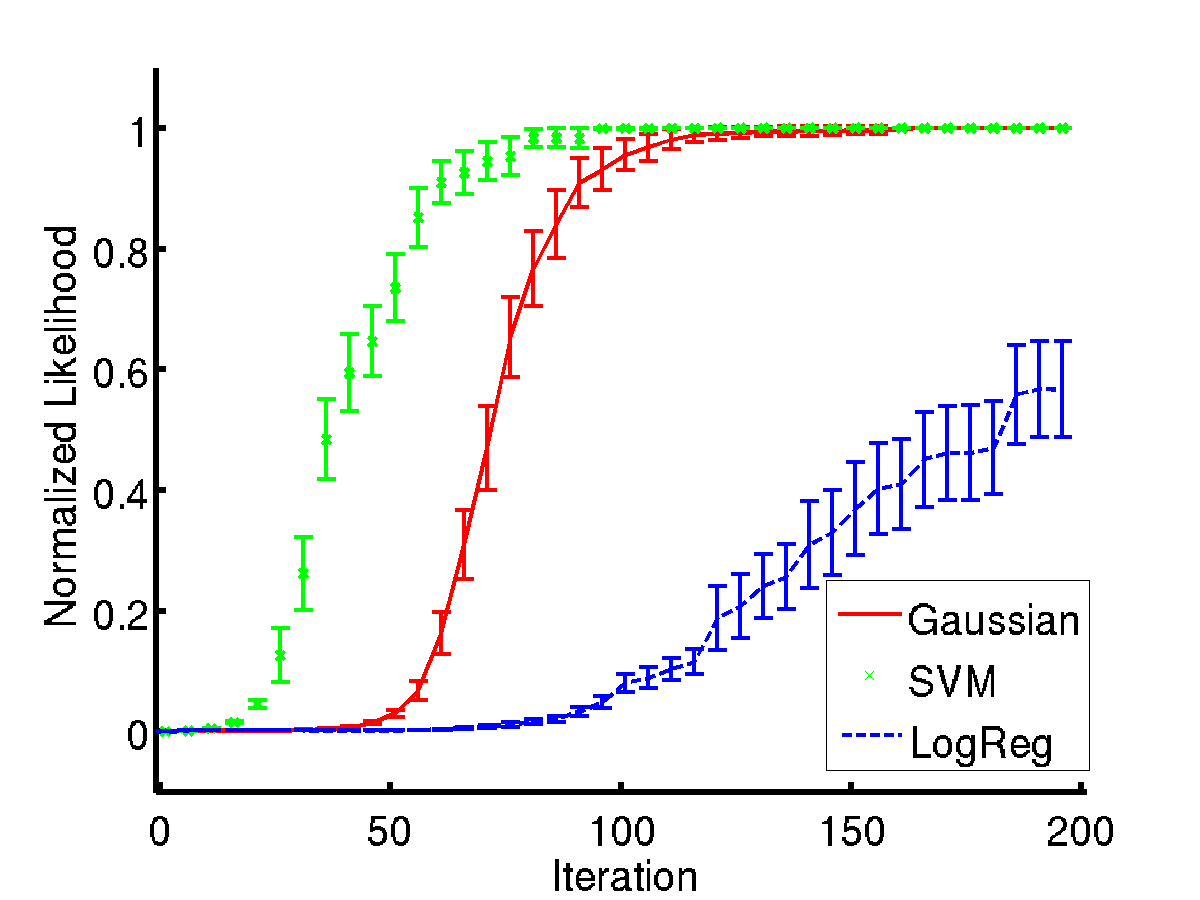
\includegraphics[width=\ww\columnwidth]{images/results/classifiers}
	\caption{Taught hypothesis normalized likelihood evolution (mean + std error) thought iteration using different kinds of classifiers. The teacher is providing feedback using one word per meaning and the agent is performing action according to $\epsilon$-greedy strategy.}
	\label{fig:FeedbackOneWord}
\end{figure}

The user is not restricted to the use of one word per meaning, table~\ref{tab:1} compares the goal normalized likelihood value after 100 iterations for feedback instructions composed of one, three and six spoken words per meaning. SVM has better performance when using one word per meaning but the Gaussian classifier has overall better results with less variance, see Table~\ref{tab:1}. 
%
\begin{table}[htbp]
\caption{Taught hypothesis normalized likelihood values after 100 iterations. Comparison for different classifiers and number of words per meaning. The gaussian classifier has overall better performances.}
\label{tab:1}
\centering
\begin{tabular}{|l|c|c|c|}
\hline
&\textbf{One word}&\textbf{Three words}&\textbf{Six words}\\\hline
\textbf{Gaussian}&1.0 (0.1)&1.0 (0.1)&0.7 (0.1)\\\hline
\textbf{SVM}&1.0 (0.0)&0.5 (0.4)&0.3 (0.4)\\\hline
\textbf{LogReg}&0.1 (0.1)&0.2 (0.3)&0.2 (0.3)\\\hline
\end{tabular}
\end{table}
%
Interestingly the Gaussian classifier learns better than the other classifiers with many words per meaning. This counter intuitive result can be explain by the high dimensionality of the space where even one gaussian can differentiate several group of clusters. As expected logistic regression performs badly due to the high dimensionality of the space. For the SVM classifier, the small number of points in each cluster is probably affecting the performances. For the following experiments, we will only consider the gaussian classifier, first because it has overall better performance but also because it is by far the faster to train and thus is the only one usable for real world and real time experiments. Indeed, in this setup, at each iteration the agent has to train 624 classifiers.
%
\begin{figure}[!htbp]
	\centering
		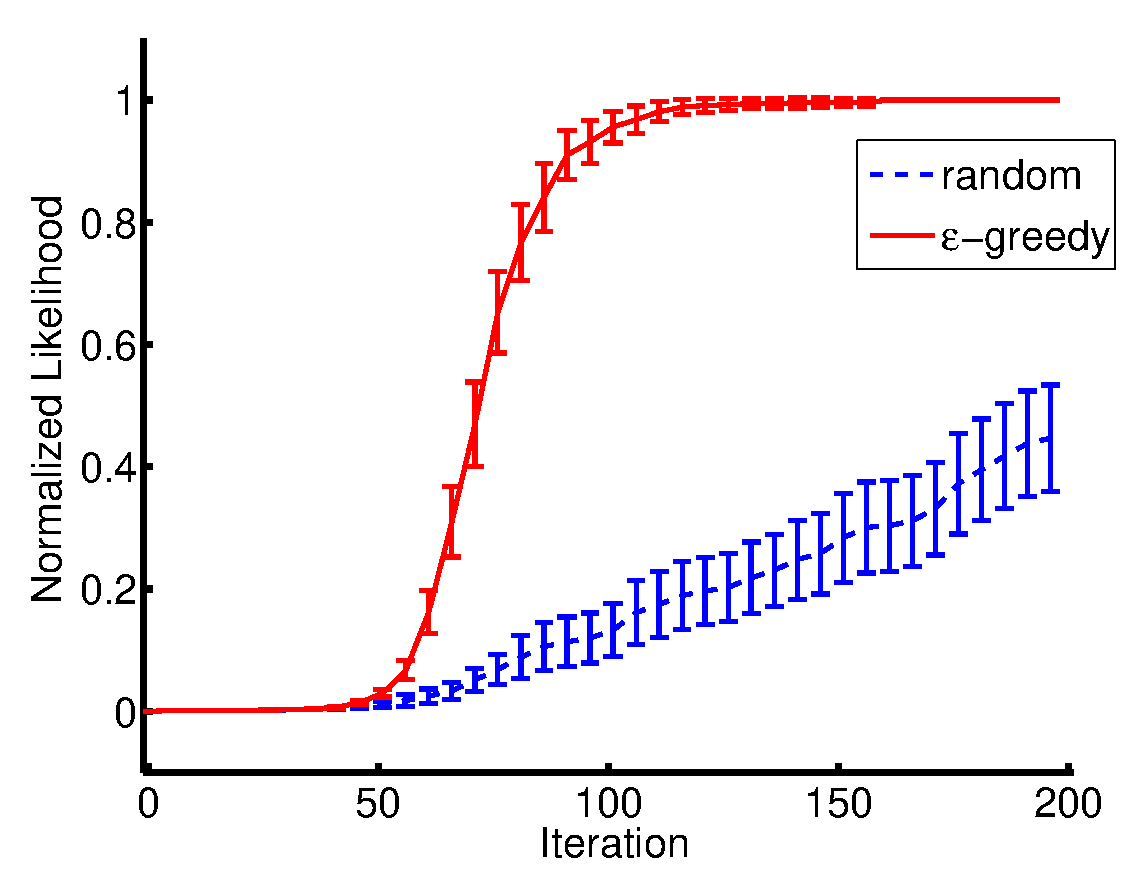
\includegraphics[width=\ww\columnwidth]{images/results/feedback}
	\caption{Taught hypothesis normalized likelihood evolution (mean + std error) thought iteration using gaussian classifier. The teacher is providing feedback using one word per meaning. The $\epsilon$-greedy action selection method learns faster than the random one. }
	\label{fig:FeedbackGaussianRdmGreed}
\end{figure}

We will now compare the impact of using different action selection methods. From Figure~\ref{fig:FeedbackGaussianRdmGreed} we can observe that $\epsilon$-greedy results in a faster learning with less variance. This method, at each step, leads the robot in the direction of the most probable goal.
In this way it will receive more diverse feedback and will visit more relevant states than what a simple random exploration would do.
%
\subsubsection{Learning guidance instructions}
%
Figure~\ref{fig:Guidance}, shows results where the teacher provides guidance instead of feedback. The number of meanings is increased from two (correct/wrong) to four (left/right/grasp/release). At each iteration the teacher first says the name of the optimal action to be performed by the robot, which then performs one action. Changes in the algorithm are described in Eq.~\ref{eq:likact}. As with feedback, the robot is able to learn the task based on guidance instructions but need more iterations to reach a perfect knowledge. Indeed, even if the robot receives more informative instructions, it now needs to classify instructions in four meanings which requires more samples to identify the clusters.  
%
\begin{figure}[!htbp]
	\centering
		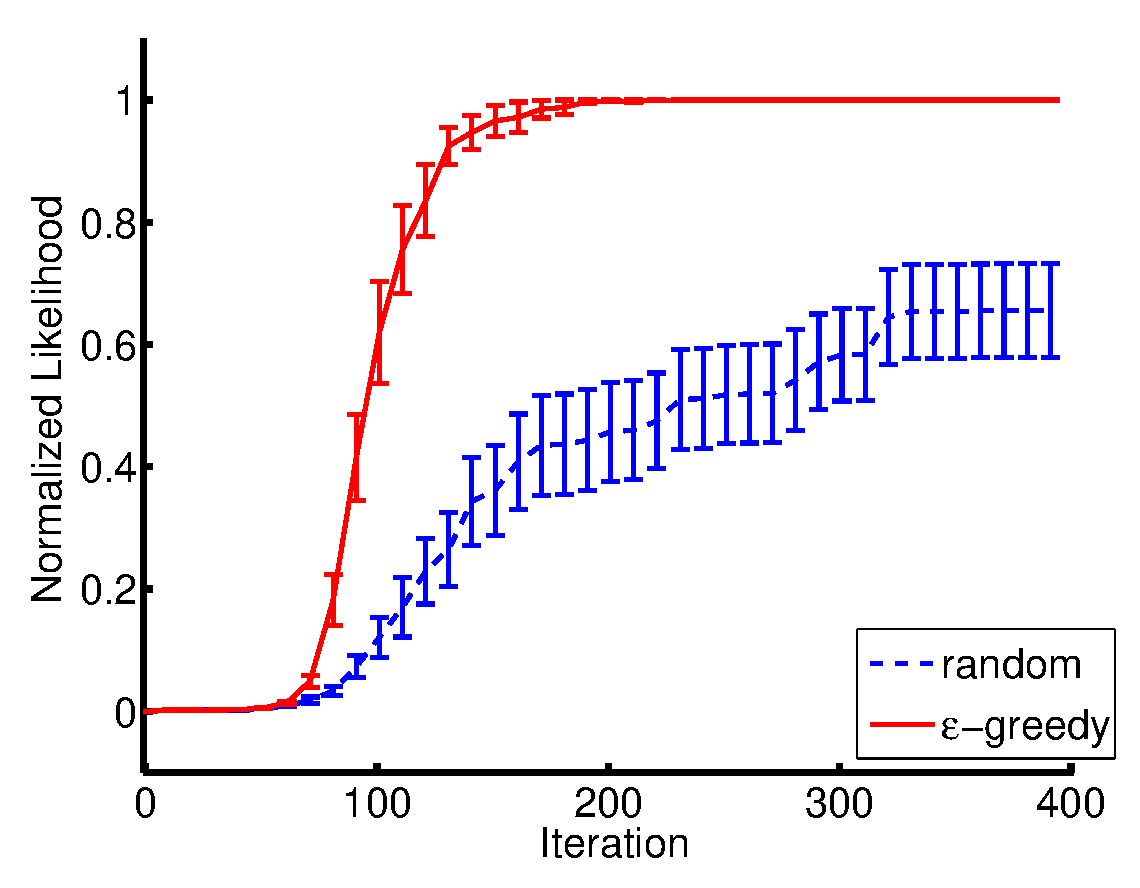
\includegraphics[width=\ww\columnwidth]{images/results/guidance}
	\caption{Taught hypothesis normalized likelihood evolution (mean + std error) thought iteration using gaussian classifier. The teacher is providing guidance using one word per action name. The $\epsilon$-greedy action selection method learns faster than the random one. }
	\label{fig:Guidance}
\end{figure}

\subsubsection{Robustness to teaching mistakes}

In results presented until now, we made the assumption that the teacher is providing feedback or guidance instructions without any mistake. But real world interactions are not perfect and people can fail in providing correct feedback. An analysis of robustness is shown in figure~\ref{fig:Noise} using feedback instructions, gaussian classifier and one word per meaning. Results with and without EM are compared to study if EM is improving robustness to teaching mistakes.
%
\begin{figure}[!htbp]
	\centering
		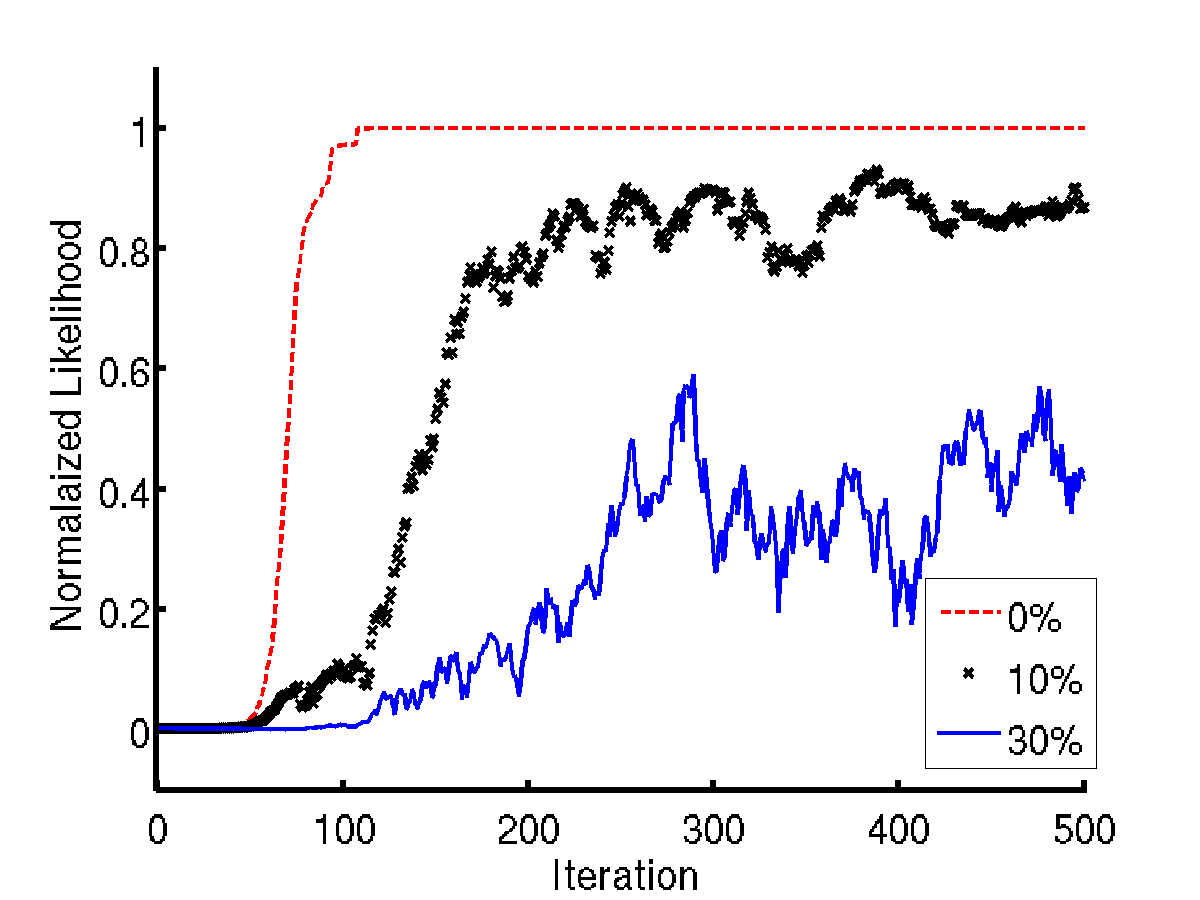
\includegraphics[width=\ww\columnwidth]{images/results/noise_no_EM}
		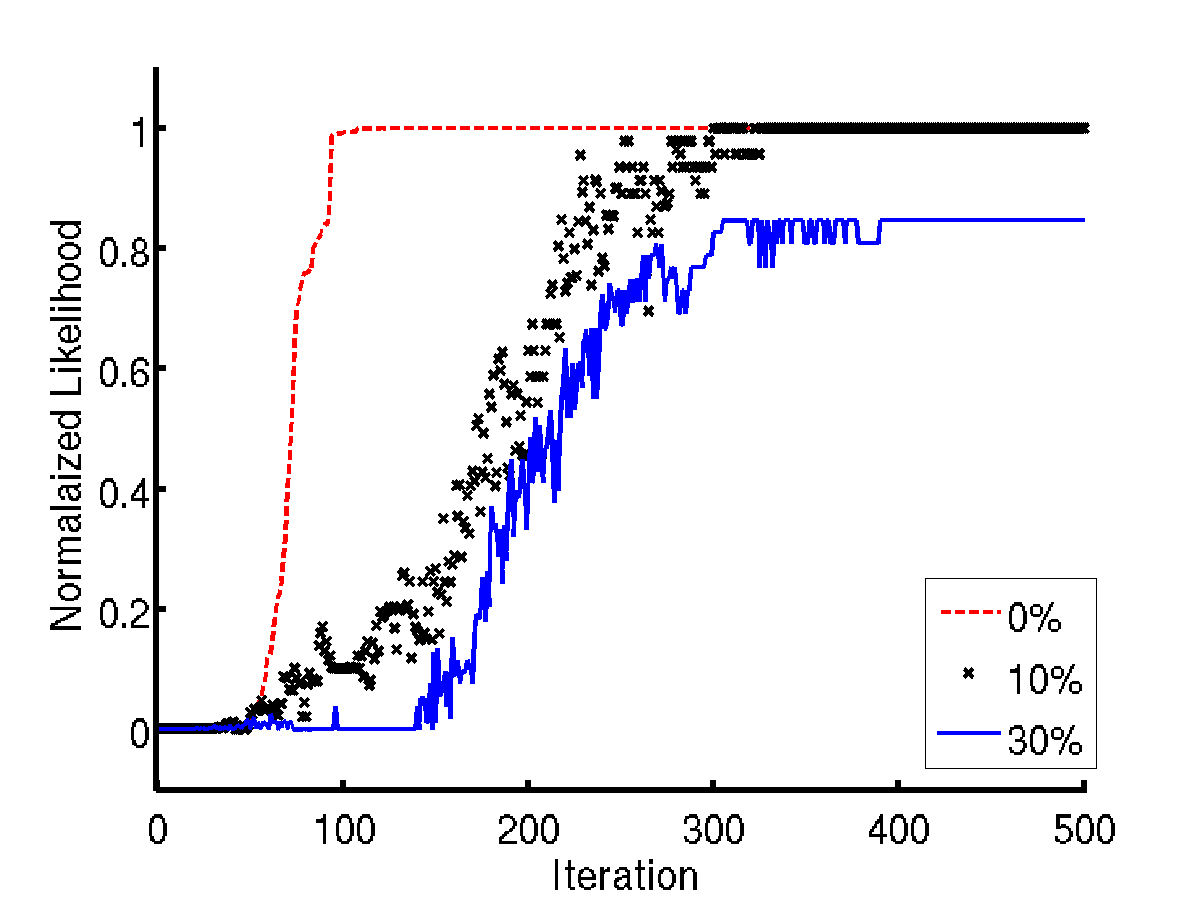
\includegraphics[width=\ww\columnwidth]{images/results/noise_with_EM}
	\caption{Taught hypothesis normalized likelihood evolution thought iteration using gaussian classifier. Comparison of one step EM (top) versus full EM (bottom). The teacher is providing feedback using one word per meaning with different percentage of mistakes. $\epsilon$-greedy action selection. Standard error has been omitted for readability reason. }
	\label{fig:Noise}
\end{figure}

We can observe that full EM is performing as expected and enables the agent to learn the task faster facing teaching mistakes. %The iterative process of EM will converge to the maximum likelihood parameters of our statistical model, reallocating teaching mistake
%Note that both technics should converge to 1 after some time.

\subsubsection{Including prior information}
\label{sec:IncludingPriorInformation}
%
Learning purely from unknown instructions is challenging for the researcher but could be restrictive for the teacher. Therefore sources of known feedback could be added, such as a green and red button, where the green button has a predefined association with a \texttt{correct} feedback meaning, as red button with a \texttt{wrong} meaning. Yet, we shall expect that even in this case, users will use more modalities than the predefined one. 
%For example, in some experiments with a robot that is explained not being capable of hearing, a majority of people are still talking to the robot \cite{rouanet2013impact}. 
In this study, the teacher still provides initially unknown spoken words feedback but can also use the red and green button as described in figure~\ref{bloc}. However, and in order to avoid possibility of direct button to instruction association, it can never use both modalities at the same time and use them alternatively with equal probability. 
%This allows us to constrain the experiment in cases where a direct mapping from button to unknown signals could not be used. 
Therefore, in average after 250 iterations the robot has received 125 known feedback and 125 unknown speech signals. This setting assumes that more information is received by the robot than the one predefined by the developer. In most systems this information is ignored but we think robots could also try learning from such unknown signals. We study three learning methods: in the first case, the robot is learning only via the known feedback, i.e. the buttons; in the second it uses only the vocal unknown signal; and in the third one, it uses both.  Figure~\ref{fig:button} shows result from this setting. 
%
\begin{figure}[!htbp]
	\centering
		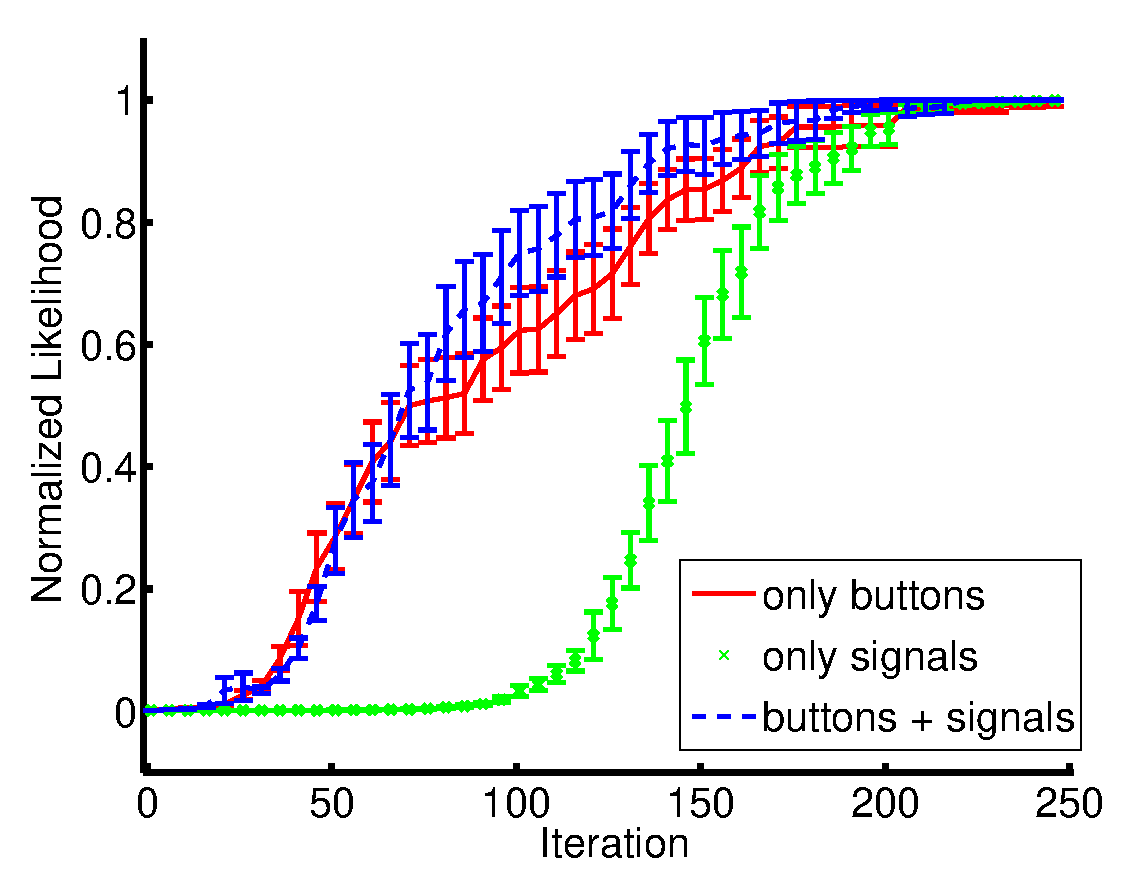
\includegraphics[width=\ww\columnwidth]{images/results/mix_button}
	\caption{Taught hypothesis normalized likelihood evolution (mean + std error) thought iteration using gaussian classifier. Comparison of using known, unknown signals and both.}
	\label{fig:button}
\end{figure}

As expected learning from known feedback is faster than with unknown, however taking advantage of different sources of information, even a priori unknown, can lead to slightly better performances than using only known information. Importantly, the instructions to meaning knowledge of the robot is updated and could therefore be reuse in further interaction.

\subsubsection{Using a real robot}
%
Statistical simulations have shown that our algorithm allows an agent to learn a task from unknown feedback in a limited amount of interactions. To bridge the gap of simulation we tested our algorithm in real interaction condition with our robotic arm. In this real experiment, the teacher is facing the robot and chooses a specific goal to reach (i.e. a specific arrangement of cube it wants the robot to build). It then decides one word to use as positive feedback and one as negative feedback and starts to teach the robot. For this experiment the word \textit{'yes'} and \textit{'no'} were respectively used for the meaning \texttt{correct} and \texttt{wrong}. Once this  experiment is terminated we keep in memory the classifier corresponding to the best task, i.e. having the higher likelihood value, and start a new experiment where the human teacher is going to use the same feedback instructions to teach a new task. But this time the spoken words are first classified as of correct or wrong meaning according to the previously learnt classifier. Therefore standard IRL algorithm can be used. We study here two things, first does our system bridges the reality gap and can we reuse information learnt from a previous experience? 
%
\begin{figure}[!htbp]
	\centering
		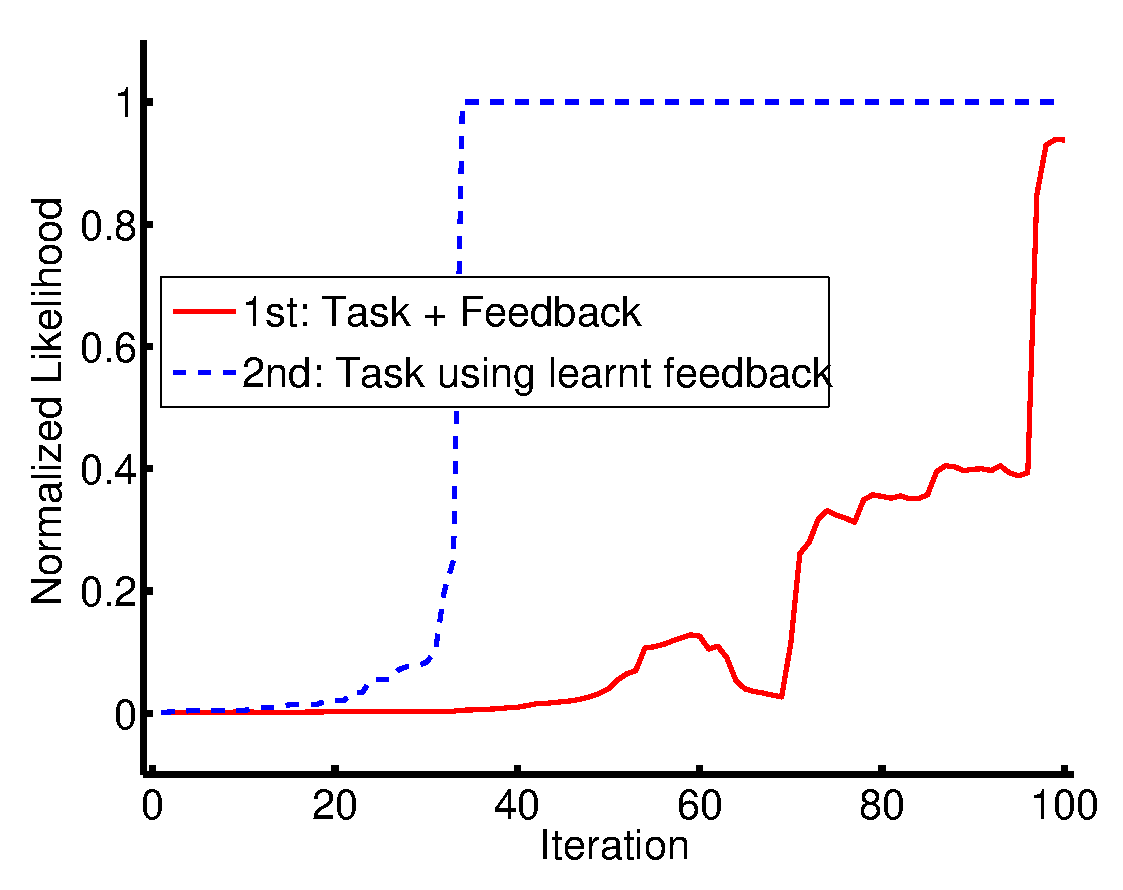
\includegraphics[width=\ww\columnwidth]{images/results/real}
	\caption{Taught hypothesis normalized likelihood evolution thought iteration using gaussian classifier.  Feedback using one word per action. $\epsilon$-greedy action selection. A first run of 100 iterations is performed where the robot learns a task from unknown feedback. Then by freezing the classifier corresponding to the best task estimate, the user teaches the robot a new task.}
	\label{Real}
\end{figure}

Figure~\ref{Real} shows results from this setting. In the first run it takes about 100 iterations for the robot to learn the task. Whereas in the second run, when reusing knowledge from the first one, the robot is able to learn a new task faster, in about 30 iterations, meaning that it has well found the two clusters in our $\mathbb{R}^{20}$ dimensional space as well as the mapping to their corresponding meanings.

%\footnote{A video explaining this experiment can be found at : \small{\url{http://flowers.inria.fr/learning-unknown-feedback.mp4}}}

\begin{comment}
\section{Results}
\label{sec:Results}

 In this section we present results from our algorithm both in simulation and with a real robotic system where we test different aspects: a) learning the associated meaning of teaching words while learning a new task, b) extend it for the case of guidance words, c) combine learning from unknown signals with pre-defined signals of known meanings, d) reuse learnt signals to meaning association for the learning of a new task.

\subsection{Experimental System}
\label{sec:ExperimentalSetup}

We construct a small size pick-and-place task with a real robot. This robot is going to be programmed using a natural language interface whose words have an unknown meaning. The robot has a prior knowledge about the distribution of possible tasks and knows how to accept teaching signals.

The interaction between the robot and the human is forced to be a turn taking social behavior, where the robot is performing an action and wait for a feedback or guidance signal to continue. This allows us to synchronize a vocal word to the corresponding pair of state and action. The experimental protocol is summarized in figure~\ref{bloc}.

\begin{figure}[!htbp]
	\centering
		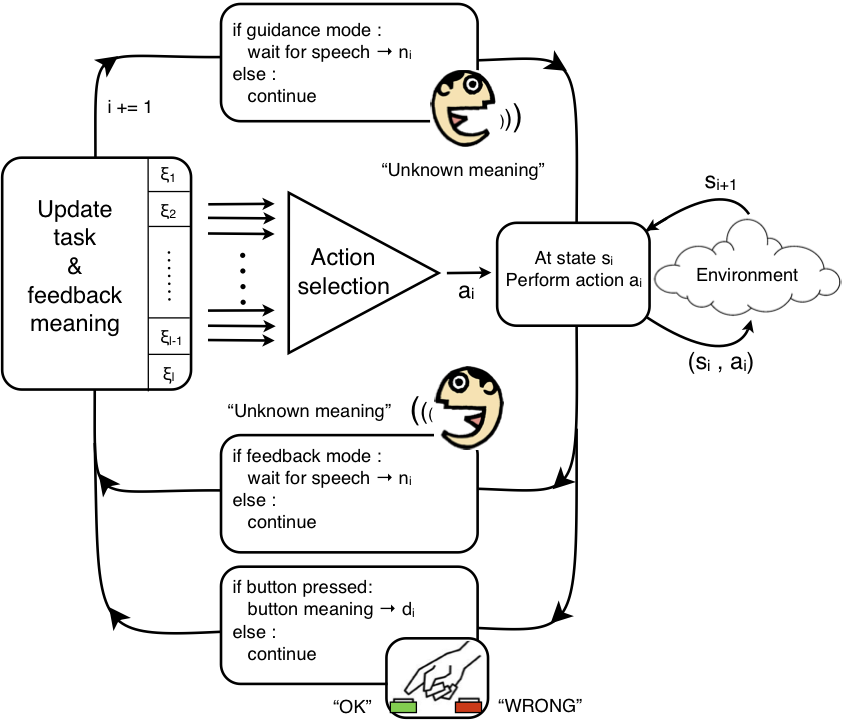
\includegraphics[width=0.9\columnwidth]{images/bloc4.png}
	\caption{Experimental protocol showing the interaction between the teacher and the learning agent. The agent has to learn a task and the meaning of the signals provided by the user, here recorded speech. The teacher can use guidance or feedback signals but has also access to buttons of known meaning for the robot.\vspace{-0.1cm}}
	\label{bloc}
	
\end{figure}

\subsubsection{Robotic System}
\label{sec:RoboticSystem}
%
We consider a six d.o.f. robotic arm and gripper that is able to grasp, transport and release cubes in four discrete positions. We used a total of three cubes that can form towers of at most two cubes.  The robot has 4 actions available: \textit{rotate left}, \textit{rotate right}, \textit{grasp cube} and \textit{release cube}. The state space is discrete and defined as the location of each object, including being on top of another or in the robot's hand. So for a set of 3 objects we have 624 different states. Figure~\ref{setup} shows the robot grasping the orange cube. The system is open loop and if a cube is moved without ``informing'' the robot, it will fail executing its plan. 

\begin{figure}[!htbp]
	\centering
		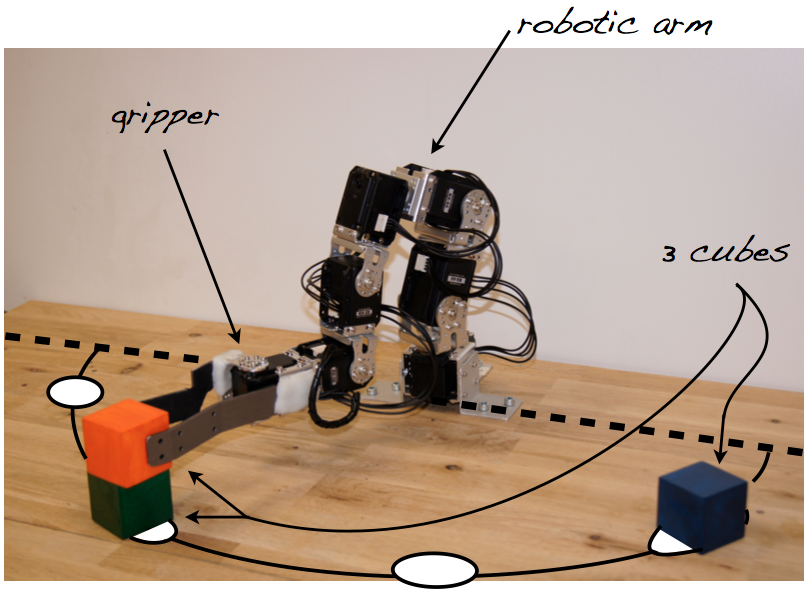
\includegraphics[width=0.6\columnwidth]{images/setup4.png}
	\caption{Robotic System. An example of cubes configuration which can be described as: \emph{
"orange cube is on top of green cube in position 3, blue cube is in position 1 and the robot is grasping the orange cube"}.\vspace{-0.5cm}}
	\label{setup}
\end{figure}

\subsubsection{Task Representation}
\label{sec:TaskRepresentation}

We assume that for a particular task $\xi$ we are able to compute a policy $\pi$ representing the optimal actions to perform in every state. One possibility is to use \textit{Markov Decision Processes} (MDP) to represent the problem \cite{sutton1998reinforcement}. From a given task $\xi$ represented as a reward function we can compute the corresponding policy using, for instance, Value Iteration. In any case, our algorithm does not make any assumption about how tasks are represented.

For this particular representation we assume that the reward function is sparse and so we can generate possible tasks by sampling sparse reward functions. Similarly to Bayesian Inverse Reinforcement Learning \cite{Ramachandran07ijcai} the robot learns the task by choosing among the possible space of rewards the most likely one. We approximate this process using a finite set of task hypothesis representing all the reward functions consisting of a unitary reward in one state and no reward in all the other. In other words the task is to reach one, yet unknown, of the 624 states of the MDP.

Under this formalism the action selection at runtime can be done in different ways. As different sampling methods can lead to different learning behaviors we will compare two different methods: random and  $\epsilon$-greedy. When following random action selection the robot does not use its current knowledge of the task and randomly select actions. Whereas with $\epsilon$-greedy method the robot performs actions according to the current belief of what the task is, i.e. following the policy corresponding to the most likely task hypothesis. The corresponding optimal action is chosen with $\epsilon$ probability, otherwise, a random one is selected. In our experiment we show only results with $\epsilon =  0.9$.

%Indeed the quality of the samples received depends on the path the robot will follow in the MDP, some can lead to very informative feedback and others to a waste of time.

\subsubsection{Speech processing}
\label{sec:SpeechProcessing}

As mentioned before, we consider speech as the modality for interacting with the robot. After each action we record the teaching word pronounced by the user. This data is mapped into a $20$ dimensional feature space using the methodology described next.  

A classical method for representing sounds is the \textit{Mel-Frequency Cepstral Coefficients} (MFCC) \cite{zheng2001comparison}. It represents a sound as a time sequence of features vector, called MFCC coefficient. Feature vector dimension can vary, in our case we used 12. Comparing sounds can then be done via \textit{Dynamic Time Warping} (DTW) between two sequences of feature vectors \cite{sakoe1978dynamic}. This distance is a measure of similarity that takes into account possible insertions and deletions in the feature sequence and is adapted for sounds comparison of different length. Each recorded vocal signal is represented as its DTW distance to 20 pre-defined base of spoken words.

By empirical test on recorded speech samples, we estimate that a number of 20 bases words were sufficient and yet a relatively high number of dimensions to deal with a variety of people and speech. This base of 20 words have been randomly selected and is composed of the words:\emph{ \footnotesize{Error, Acquisition, Difficulties, Semantic, Track, Computer, Explored, Distribution, Century, Reinforcement, Almost, Language, Alone, Kinds, Humans, Axons, Primitives, Vision, Nature, Building}}.

\subsubsection{Classification System for the Symbol Model}
\label{sec:classifiers}

As explained in section \ref{sec:Algorithm}, any standard machine learning classifier can be used for approximating the symbol model. If such classifier is not able to use probabilistic labels then the maximization step of the EM algorithm is approximated in Eq. \ref{eq:F} with a hard thresholds for $z_i^{\xi}$. We then have to rely on the generalization performances of the classifier. Indeed, if the classification algorithm is overfitting the data then no differences can be found between the different hypotheses. The only required characteristic is the ability to output a confidence on the class prediction, i.e. a probability for $n_i$ of being associated to each meaning.

In this study we decided to compare three classifiers for the symbol learning:
\begin{itemize}
\item Gaussian Bayesian Classifier: Computing the weighted mean $\mu$ and covariance matrix $\Sigma$, the usual equations for gaussian mixture hold.
\item Support Vector Machine (SVM): Using a RBF kernel with $\sigma = 1000$ (high dimensional space) and $C = 0.1$.  For SVM probabilistic prediction refer to \cite{platt1999probabilistic}.
\item Logistic regression: The predictive output value ($\in [0,1]$) is used as a measure of confidence. This algorithm is usually not well suited for high dimensional spaces as the euclidean distances are huge in such spaces.
\end{itemize}

\subsection{Experimental Results}
\label{sec:ExperimentalResults}

Experiments presented in this section follow the protocol described in figure~\ref{bloc}, where by turn the agent perform one action and wait for teaching signals from the teacher. Teacher is providing a signal after each action of the robot. We first present a set of statistical simulated experiments using the same MDP as for the real word experiment. We start by assuming that the teacher is providing feedback without any mistake, therefore only the noise in the signals remain. We compare first the different classifiers, and then the performances of $\epsilon$-greedy versus random action selection methods both for feedback and guidance mode. Later, we present an analysis of robustness to teacher mistakes while comparing one step EM with full EM. Last simulated experiment studies the case where the teacher has also access to buttons of known meaning. Finally, we show the result of one real word experiment where we study how signals knowledge learnt in a first run can be used in a second one to learn more efficiently.

In order to stay as close as possible to the real world setup, data used as teaching signals in simulation are recorded spoken words mapped to our 20 dimensional space. Such words consist of:  \emph{\small{Good, Bad, Left, Right, Grasp, UnGrasp, Yes, No, Clockwise, CounterClockwise, Hold, PutDown}}, we remember that their everyday meaning have no relation with their meaning in the experiment, e.g. \emph{``Left''} could be used to give a positive feedback. We recorded enough samples of each word to avoid using the same sample twice in the same run.

All results report averages of 20 executions of the algorithm with different start and goal states. By normalizing the sum of all likelihoods estimate ($q_1,\ldots,q_l$) to 1, we obtain the probability of each particular task hypothesis to represent the task to learn. The normalized likelihood of the task to be learnt $q(\xi^*)$ is our measure of learning progress.

\subsubsection{Learning feedback signals}

In this experiment we assume that the robot does not know the words being spoken by the teacher and it does not know the task either. The robot will, simultaneously, learn the task and map the words that is recording into a binary feedback signal.

The results comparing the different classification methods are shown in Figure~\ref{fig:FeedbackOneWord}. Action selection is done $\epsilon$-greedy. Note that after 200 iterations all three methods learn the task, i.e. the normalized goal likelihood value is greater than 0.5, meaning that the sum of all the others is inferior to 0.5. Logistic regression provides the worse results in terms of convergence rate and variance. \vspace{-0.3cm}

\begin{figure}[!htbp]
	\centering
		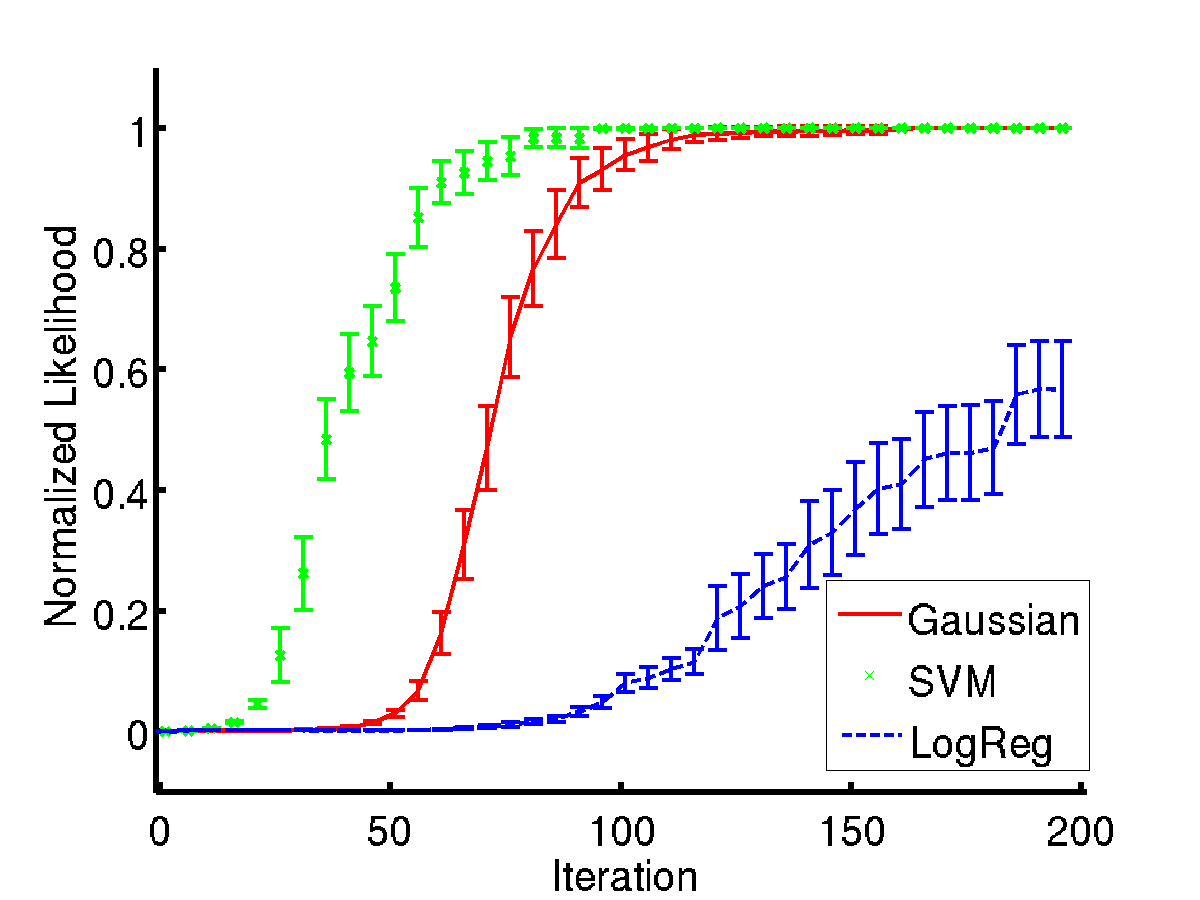
\includegraphics[width=\ww\columnwidth]{images/results/classifiers}
	\caption{Goal normalized likelihood evolution (mean + std error) thought iteration using different kinds of classifiers. The teacher is providing feedback using one word per meaning and the agent is performing action according to $\epsilon$-greedy method. \vspace{-0.1cm} }
	\label{fig:FeedbackOneWord}
\end{figure}

The user is not restricted to the use of one word per meaning, table~\ref{tab:1} compares the goal normalized likelihood value after 100 iterations for feedback signals composed of one, three and six spoken words per meaning. SVM has better performance when using one word per meaning but the Gaussian classifier has overall better results with less variance, see Table~\ref{tab:1}. 

\begin{table}[htbp]
\caption{\scriptsize{Mean and variance goal normalized likelihood values after 100 iterations. Comparison for different classifiers and number of words per meaning. The gaussian classifier has overall better performances.}}
\label{tab:1}
\centering
\begin{tabular}{|l|c|c|c|}
\hline
&\textbf{One word}&\textbf{Three words}&\textbf{Six words}\\\hline
\textbf{Gaussian}&1.0 (0.1)&1.0 (0.1)&0.7 (0.1)\\\hline
\textbf{SVM}&1.0 (0.0)&0.5 (0.4)&0.3 (0.4)\\\hline
\textbf{LogReg}&0.1 (0.1)&0.2 (0.3)&0.2 (0.3)\\\hline
\end{tabular}

\end{table}

Interestingly the Gaussian classifier learns better than the other classifiers with many words per meaning. This counter intuitive result can be explain by the high dimensionality of the space where even one gaussian can differentiate several group of clusters. As expected logistic regression performs badly due to the high dimensionality of the space. For the SVM classifier, the small number of points in each cluster is probably affecting the performances. For following experiments, we will only consider the gaussian classifier, first because it has overall better performance but also because it is by far the faster to train and thus is the only one usable for real world and real time experiments. Indeed, in this setup, at each iteration the agent has to train 624 classifiers.\vspace{-0.2cm}

\begin{figure}[!htbp]
	\centering
		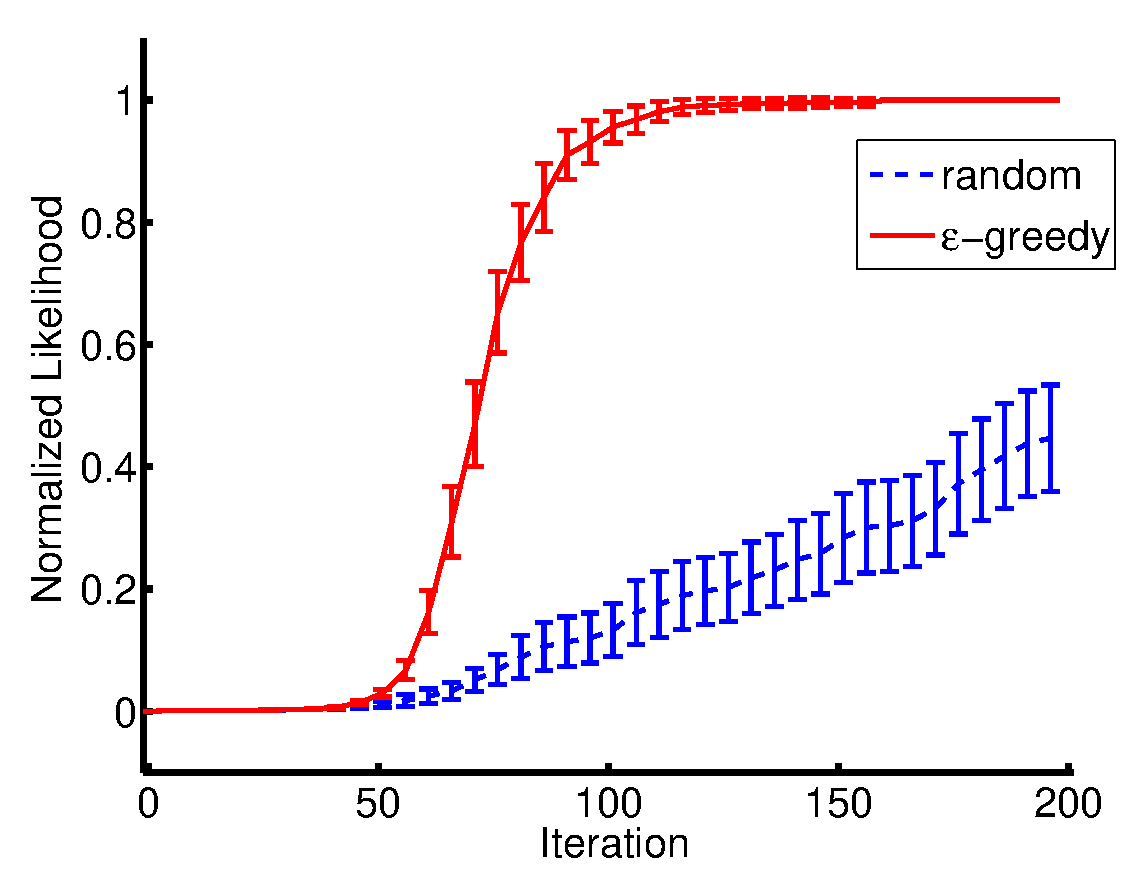
\includegraphics[width=\ww\columnwidth]{images/results/feedback}
	\caption{Goal normalized likelihood evolution (mean + std error) thought iteration using gaussian classifier. The teacher is providing feedback using one word per meaning. The $\epsilon$-greedy action selection method learns faster than the random one. \vspace{-0.2cm}}
	\label{fig:FeedbackGaussianRdmGreed}
\end{figure}

We will now compare the impact of using different action selection methods. From Figure~\ref{fig:FeedbackGaussianRdmGreed} we can observe that $\epsilon$-greedy results in a faster learning with less variance. This method, at each step, leads the robot in the direction of the most probable goal.
In this way it will receive more diverse feedback and will visit more relevant states than what a simple random exploration would do.

\subsubsection{Learning guidance signals}

Figure~\ref{fig:FeedbackOneWord}, shows results where the teacher provides guidance instead of feedback. The number of meaning is increased from two (correct/wrong) to four (left/right/grasp/release). At each iteration the teacher first says the name of the optimal action to be performed by the robot, which then performs one action. Changes in the algorithm are described in Eq.~\ref{eq:likact}. As with feedback, the robot is able to learn the task based on guidance signals but need more iterations to reach a perfect knowledge. Even if the robot receives more informative signals, it now needs to classify them in four different meanings which requires more samples. \vspace{-0.1cm}

\begin{figure}[!htbp]
	\centering
		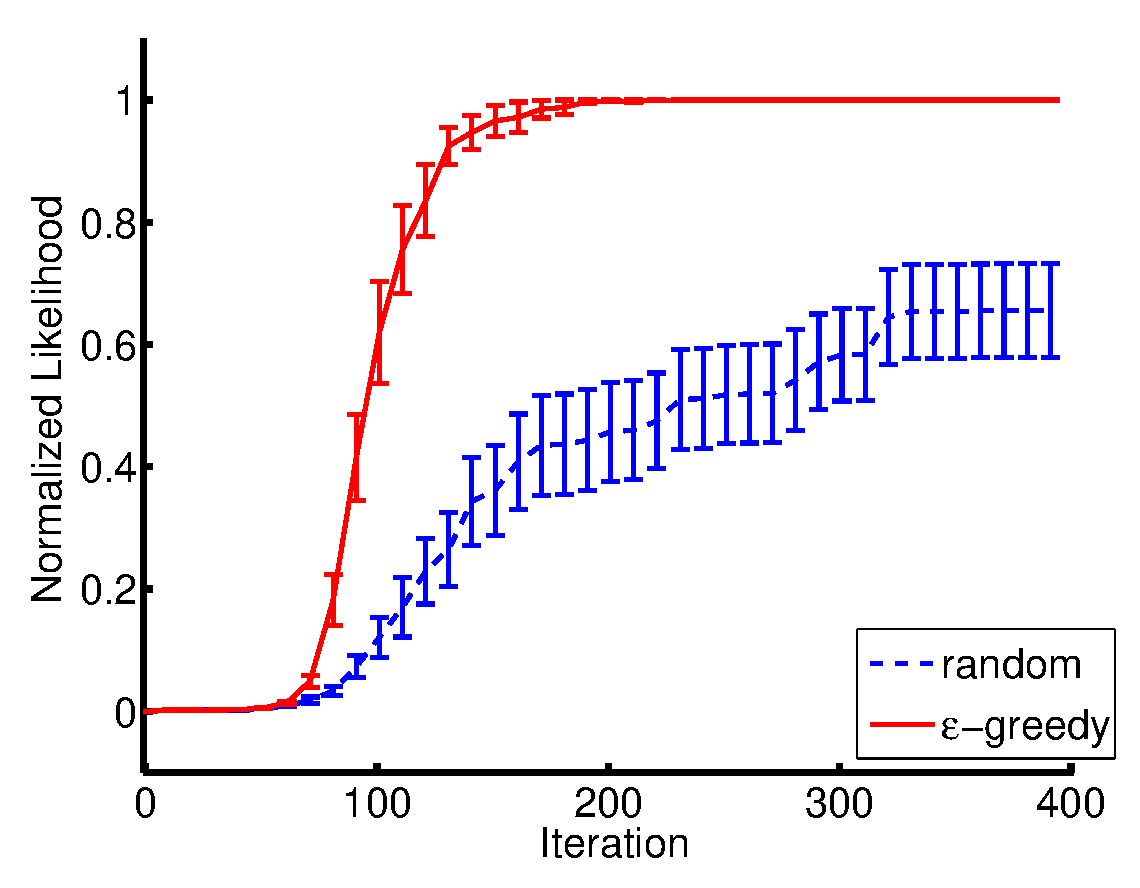
\includegraphics[width=\ww\columnwidth]{images/results/guidance}
	\caption{Goal normalized likelihood evolution (mean + std error) thought iteration using gaussian classifier. The teacher is providing guidance using one word per action name. The $\epsilon$-greedy action selection method learns faster than the random one. \vspace{-0.1cm}}
	\label{fig:Guidance}
\end{figure}

\subsubsection{Robustness to teaching mistake}

In results presented until now, we made the assumption that the teacher is providing feedback or guidance signals without any mistake. But real world interactions are not perfect and people can fail in providing correct feedback. An analysis of robustness is shown in figure~\ref{fig:Noise} using feedback signals, gaussian classifier and one word per meaning. Results with one step EM and full EM are compared to study if  full EM is improving robustness to teaching mistakes. \vspace{-0.2cm}

\begin{figure}[!htbp]
	\centering
		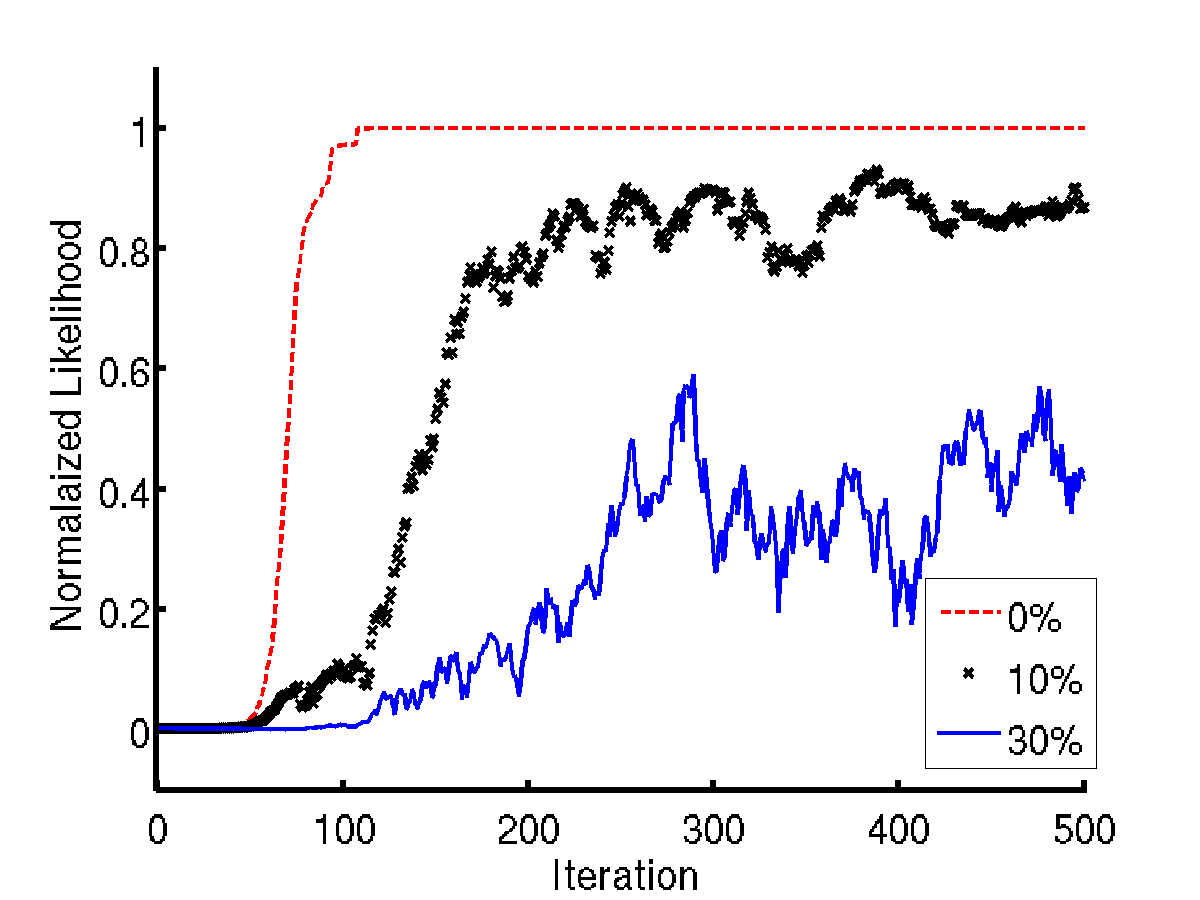
\includegraphics[width=0.60\columnwidth]{images/results/noise_no_EM}
		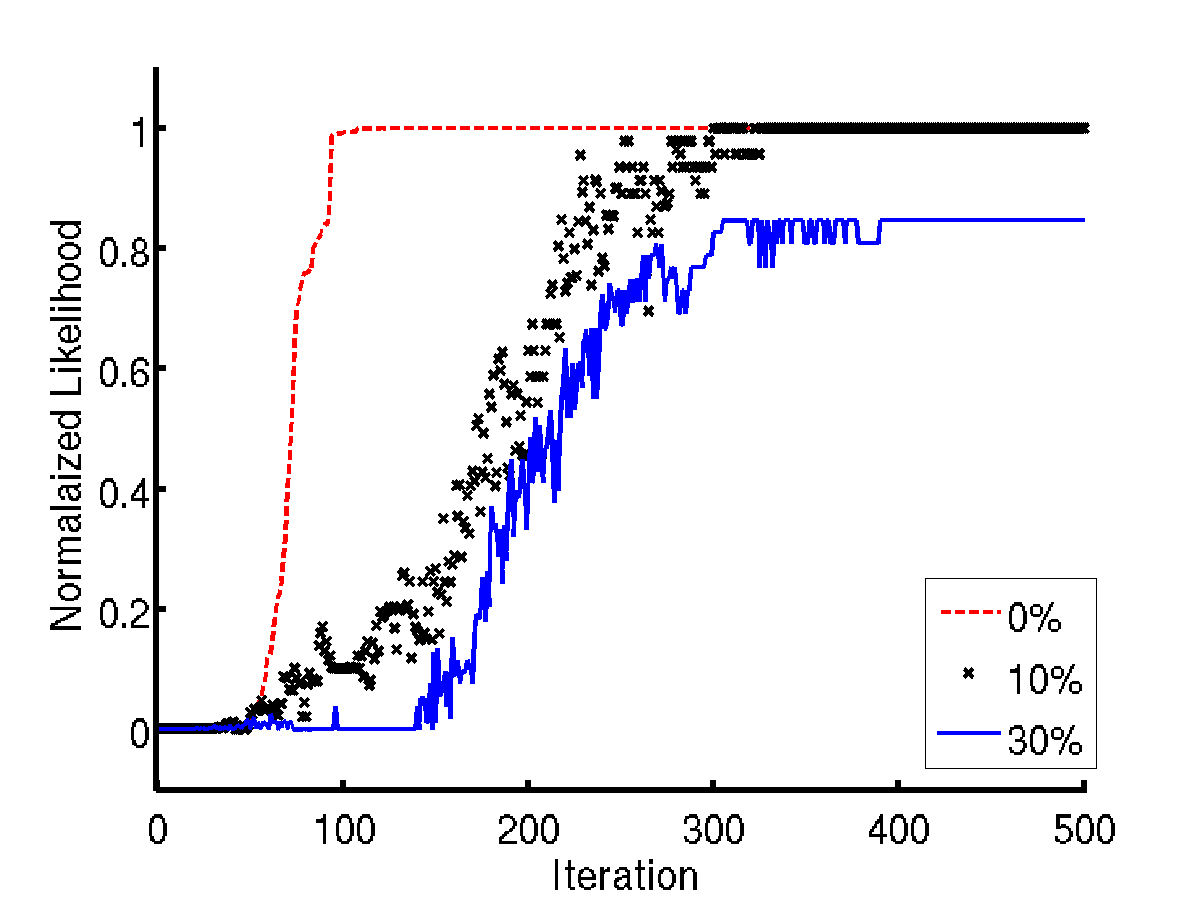
\includegraphics[width=0.60\columnwidth]{images/results/noise_with_EM}
	\caption{Goal normalized likelihood evolution thought iteration using gaussian classifier. Comparison of one step EM (top) versus full EM (bottom). The teacher is providing feedback using one word per meaning with different percentage of mistake. $\epsilon$-greedy action selection. Standard error has been omitted for readability reason. \vspace{-0.4cm}}
	\label{fig:Noise}
\end{figure}

We can observe that full EM is performing as expected and enables the agent to learn the task faster facing teaching mistake.
%Note that both technics should converge to 1 after some time.

\subsubsection{Including prior information}
\label{sec:IncludingPriorInformation}

Learning purely from unknown teaching signals is challenging for the researcher but could be restrictive for the teacher. Therefore sources of known feedback could be added, such as a green and red button. Where the green button has a predefined association with a \texttt{correct} feedback meaning, as red button with a \texttt{wrong} meaning. Yet, we shall expect that even in this case, users will use more modalities than the predefined one. 
%For example, in some experiments with a robot that is explained not being capable of hearing, a majority of people are still talking to the robot \cite{rouanet2013impact}. 
In this study, the teacher still provides initially unknown spoken words feedback but can also use the red and green button as described in figure~\ref{bloc}. However, and in order to avoid possibility of direct button to signal association, it can never use both modalities at the same time and use them alternatively with equal probability. 
%This allows us to constrain the experiment in cases where a direct mapping from button to unknown signals could not be used. 
Therefore, in average after 250 iterations the robot has received 125 known feedback and 125 unknown speech signals. This setting assumes that more information is received by the robot than the one predefined by the developer. In most systems this information is ignored but we think robots could also try learning from such unknow signals. We study three learning methods: in the first case, the robot is learning only via the known feedback, i.e. the buttons; in the second it uses only the vocal unknown signal; and in the third one, it uses both.  Figure~\ref{fig:button} shows result from this setting. \vspace{-0.2cm}

\begin{figure}[!htbp]
	\centering
		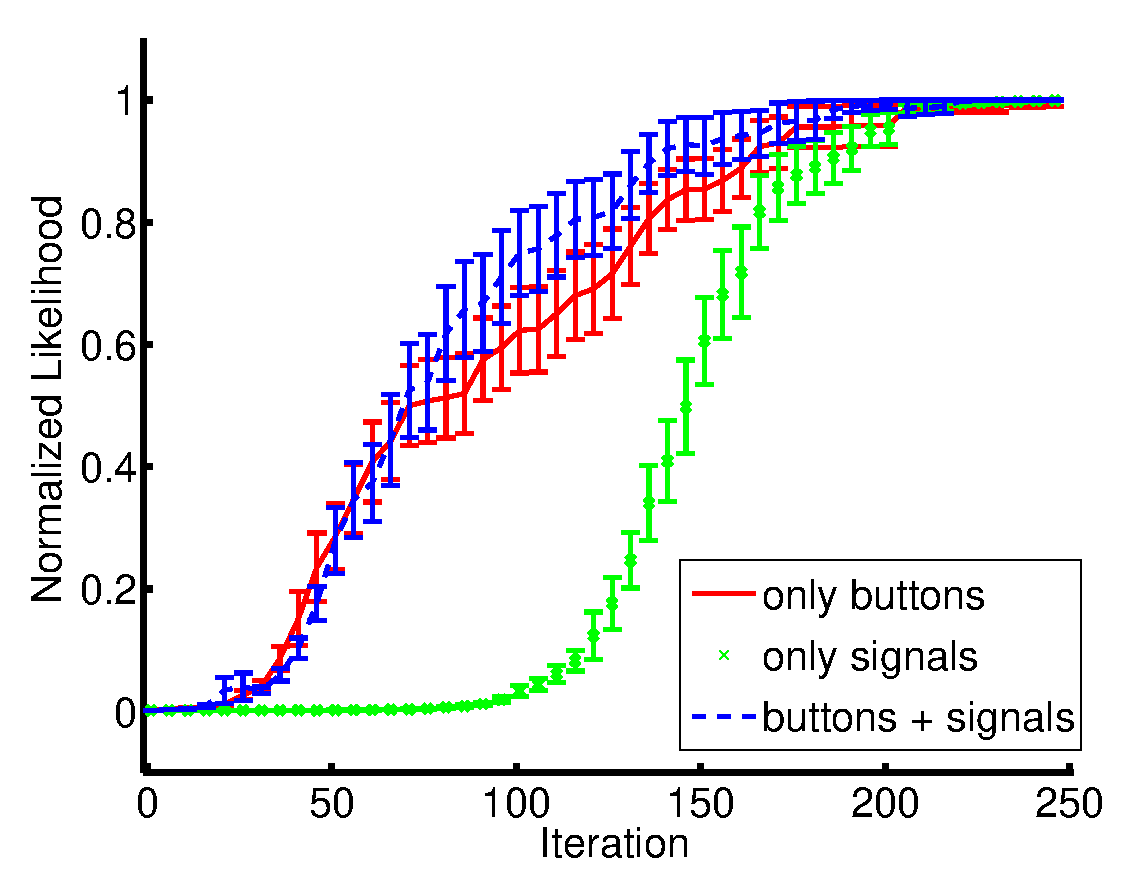
\includegraphics[width=\ww\columnwidth]{images/results/mix_button}
	\caption{Goal normalized likelihood evolution (mean + std error) thought iteration using gaussian classifier. Comparison of using known, unknown signals and both. Standard deviation have been omitted for readability.\vspace{-0.1cm}}
	\label{fig:button}
\end{figure}

As expected learning from known feedback is faster than with unknown, however taking advantage of different sources of information, even a priori unknown, can led to slightly better performances than using only known information. Importantly, the signals to meaning knowledge of the robot is updated and could therefore be reuse in further interaction.

\subsubsection{A real word experiment}

Statistical simulations have shown that our algorithm allows an agent to learn a task from unknown feedback in a limited amount of interactions. To bridge the gap of simulation we tested our algorithm in real interaction condition with our robotic arm. In this real experiment, the teacher is facing the robot and chooses a specific goal to reach (i.e. a specific arrangement of cube he wants the robot to build). He then decides one word to use as positive feedback and one as negative feedback and starts to teach the robot. Once this  experiment is terminated we keep in memory the classifier corresponding to the best task, i.e. having the higher likelihood value, and start a new experiment where the human teacher is going to use the same feedback signals to teach a new task. But this time the spoken words are first classified as of correct or wrong meaning according to the previously learnt classifier. Therefore standard IRL algorithm can be used. We study here two things, first does our system bridges the reality gap and can we reuse information learnt from a previous experience? 

\begin{figure}[!htbp]
	\centering
		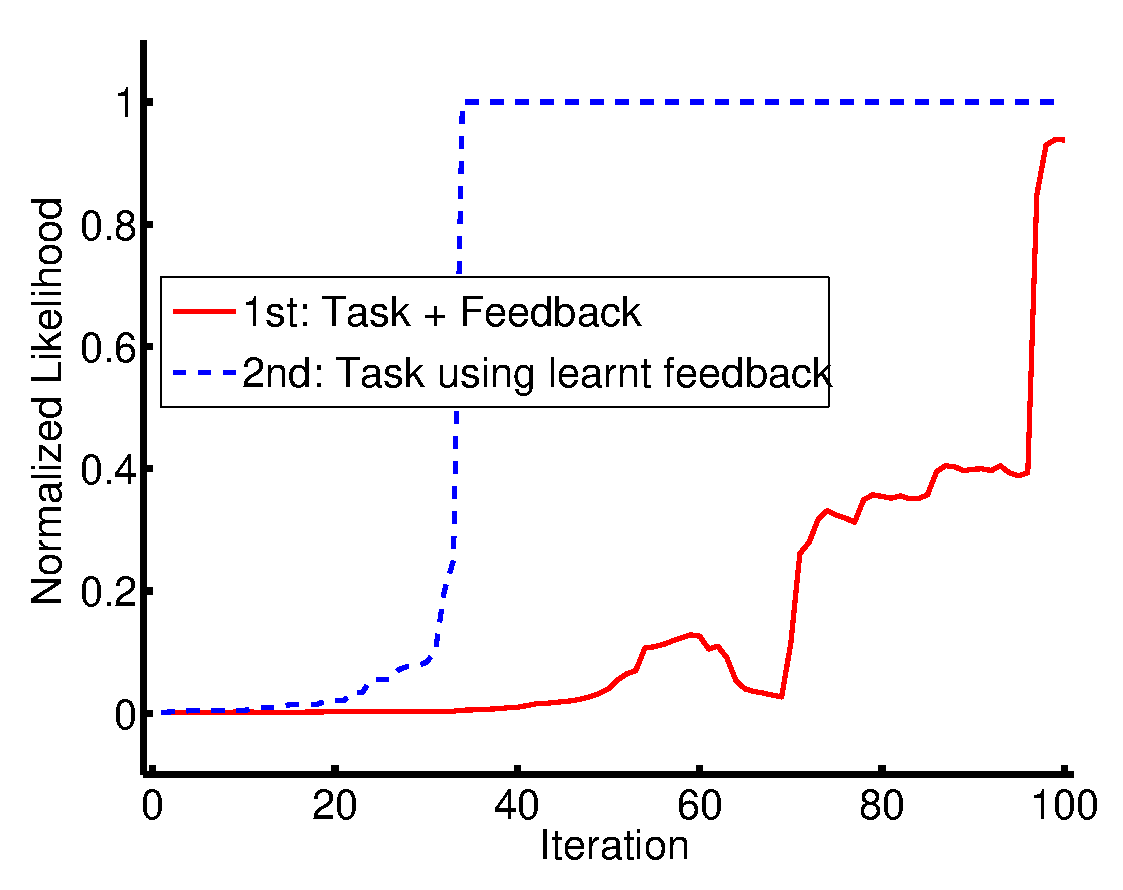
\includegraphics[width=\ww\columnwidth]{images/results/real}
	\caption{Goal normalized likelihood evolution thought iteration using gaussian classifier.  Feedback using one word per action. $\epsilon$-greedy action selection. A first run of 100 iterations is performed where the robot learns a task from unknown feedback. Then by freezing the classifier corresponding to the best task estimate, the user teaches the robot a new task.\vspace{-0.5cm}}
	\label{Real}
\end{figure}

Figure~\ref{Real} shows results from this setting. In the first run it takes about 100 iterations for the robot to learn the task. Whereas in the second run, when reusing knowledge from the first one, the robot is able to learn a new task faster, in about 30 iterations, meaning that it has well found the two clusters in our $\mathbb{R}^{20}$ dimensional space as well as the mapping to their corresponding meanings.

%\footnote{A video explaining the all process can be found at : \small{\url{http://flowers.inria.fr/learning-unknown-feedback.mpg}}}

\end{comment}
